\section{Crawling based on Reinforcement Learning}\label{section:solution}

Our goal in efficient crawling is to retrieve as many targets as possible at minimal cost, without prior knowledge of the website's size or structure. We hypothesize that \emph{an edge's label} $\lambda$ (its tag path in the page containing the hyperlink) \emph{can be used to learn which edges leads to target-rich pages}. Obtaining and leveraging such insignhts require both \emph{exploration} (to find promising paths) and \emph{exploitation} (to retrieve targets), which we achieve via \emph{reinforcement learning} (RL)~\cite{sutton2018reinforcement}. 
Below, we present the environment (states and actions) of our crawling task (Sec.~\ref{subsection:states_actions}), and the learning algorithm (or \emph{ agent}) that evolves in it (Sec.~\ref{subsection:group-links}).
We describe the URL classifier we use to compute the agent's rewards in 
Sec.~\ref{subsection:url_classifier}, and the overall crawling algorithm in Sec.~\ref{subsection:crawling_algorithm}.


\subsection{Environment: States and Actions}\label{subsection:states_actions}

In RL, an \emph{agent} evolves in an \emph{environment}. It starts from an initial \emph{state}, where it can choose among a set of \emph{actions}. Each \emph{action} leads to a new \emph{state}, where other actions can be chosen. Each choice leads to a \emph{reward}. The  goal of the agent is to learn a \emph{policy} (a mapping from states to actions), that maximizes the total reward. This model is known as a \emph{Markov Decision Process} (MDP) \cite{howard1960dynamic}.
For our crawler, one might consider using ``the currently crawled webpage'' as \emph{state}. However, this is not suitable: the current webpage does not reflect previous choices, as it may be reachable via multiple paths. Also, an efficient crawler should not visit any webpage twice, whereas learning supposes multiple visits to a state to refine and then leverage information learned in that state.

To keep the model simple and lightweight (see Sec.~\ref{section:related_work} for discussion), we use a \textbf{single-state model}, where the agent is perpetually in exactly only one state. What matters then is only the set of \emph{actions} that the agent can follow at each crawl step. Intuitively, an action is to navigate along a link. We delve into action details below.


\subsection{Grouping Links into Actions}\label{subsection:group-links}

Following our hypothesis that \emph{links with similar labels (tag paths) have similar values}, i.e., likelihood of leading to targets, we model an action as \emph{a group
	of similar links}, with the semantics that taking the action amounts to
      crawling along one of these links.

Each link is labeled with its tag path, so we need a measure of similarity between tag paths.
To that effect, we represent each tag path by a \emph{numerical bag-of-words (BoW) vector~$p$}, over the $n$-grams vocabulary built from all tag paths encountered so far.
Note that $n$-grams preserve the order of HTML node names appearing in tag paths; in our context, this order is significant (as Sec.~\ref{sec:results} confirms).
Since the $n$-grams vocabulary is \emph{dynamically} built during the crawl, BoW vectors for tag paths encountered at different times have different lengths. To still compute distances between them, we first \emph{project each tag path into a fixed-dimensional vector} of size $D = 2^m$ for a chosen $m > 0$. We do this as follows:

\begin{asparaenum}
	\item We fix a \emph{hash function} $h: x\mapsto\left\lfloor\frac{(\Pi \times x) \mod 2^w}{2^{w-m}}\right\rfloor$ which maps
	any integer $x$ to a number between $0$ and $D-1$. Its parameters $\Pi$ (a large prime number) and $w$ are fixed, and chosen such that $w>m$. 
	\item  Calling~$h$ on each position between $0$ and $d-1$, where $d$ is
	the length of the BoW vector~$p$, maps it to a new position between $0$
  and $D-1$. This enables us to transform $p$ into a $D$-dimensional
  $p_D$ vector, where for every $0\leq i<d$, $p_D\left[h(i)\right]=p\left[i\right]$.
	\item Potential collisions of $h$ (i.e., $i_1\neq i_2$ with
	$h\left(i_1\right)=h\left(i_2\right)$) are resolved by setting $p_D\left[h(i_1)=h(i_2)\right]$
	to the \emph{mean} of all elements of $p$, at positions which collide with
	$i_1,i_2$. 
	Positions $0\le j<D$ not hit by any $i$ ($h(i)\ne j$ for all $0\le i<d$) are set to $p_D[j]=0$. This happens, e.g., at the beginning of the crawl, when the set of HTML element names seen so far is small (thus $d$ is small).
\end{asparaenum}


Figure~\ref{fig:sample-link-vectors} illustrates tag path
projection for 
$D=2^m=4$, $w=11$ and $\Pi=766\,245\,317$. At iteration~$k$, the 2-gram vocabulary contains $d_k=5$ elements
(including special tokens \texttt{BOS} and \texttt{EOS} denoting
beginning and end of stream). At iteration~$k+1$, a new tag path is
vectorized into a 2-gram vector of dimension~$10$, and the
vocabulary is updated accordingly, totaling 
$d_{k+1}=11$ elements. 
From it, we compute the
$d_{k+1}$-dimensional BoW vector $p_{k+1}$.
The hash function~$h$ maps
each input dimension $i \in
\left\{0,\dots,d_{k+1}{-}1\right\}$ to
$\left\{0,\dots,D{-}1\right\}$, e.g.,
$h(2)=\left\lfloor \frac{(766\,245\,317 \times 2) \mod 2048}{512}
\right\rfloor=1$. 
Collisions can occur, e.g.,
$h(4)$$=$$h(8)$$=$$h(9)$$=$$3$, so ${p_D}_{k+1}[3]$$=$
$\frac{p_{k+1}[4] + p_{k+1}[8] + p_{k+1}[9]}{3}$$\approx$$0.67$. This yields a 4-dimensional ${p_D}_{k+1}$.


\begin{figure}[t!]
	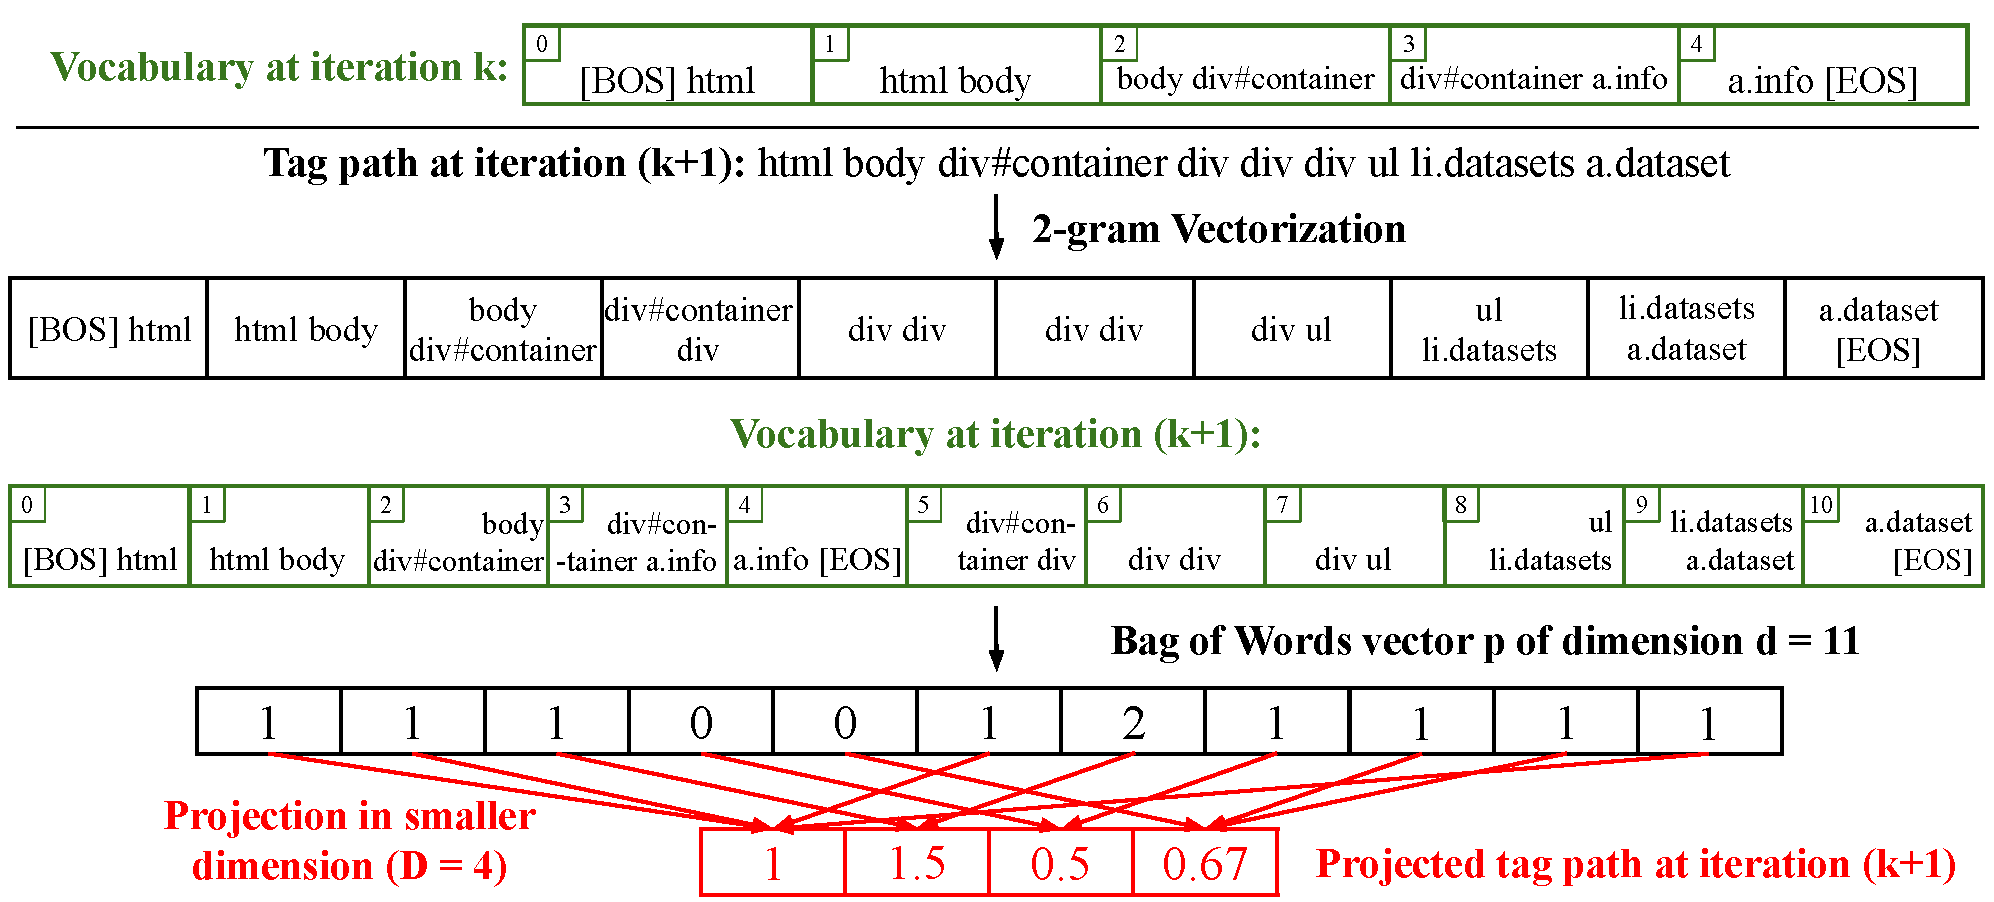
\includegraphics[width=1\linewidth]{plots/example_dom_path_vector_computation}
	\caption{Mapping of a tag path into a fixed-size vector.\label{fig:sample-link-vectors}}
\end{figure}

Our next task is to find, for each projected tag path $p_D$, the nearest action $a_c$  among all known actions~$A$.
Conceptually, an action is an evolving cluster of similar
tag paths with a centroid: the mean of all projected tag paths.
For efficiency, we only store the centroid, which updates as the action's set of tag paths evolves.

Algorithm \ref{alg:url_mapping} computes the nearest action of each $p_D$ if it is close enough; otherwise, it creates a new action.
Action centroids are stored in a \emph{Hierarchical Navigable Small Worlds} (HNSW)~\cite{malkov2018efficient} index~$\mathcal{I}$, chosen for its highly efficient updates of centroids as new tag paths join. While maintaining and querying this index might be costly in CPU time, it is negligible compared to  crawl time (waiting between two requests, or webpages download). The index also estimates the \emph{cosine similarity}
between $p_D$ and its closest centroid: if above a
threshold $\theta$, the tag path is added to the action; 
otherwise, a new action composed of only $p_D$ is created. As our experiments show (Sec.~\ref{sec:results}), the choice of $\theta$ significantly impacts  the agent performance. In extreme cases, $\theta=0$ groups all tag paths into a single action, preventing learning as the agent selects paths randomly, whereas $\theta=1$ creates a separate action for each path, so the agent only explores and never exploits. A useful threshold balances enough actions to separate interesting from uninteresting paths while still enabling learning and exploitation.

\begin{algorithm}[t!]
	\caption{Finding the action for a hyperlink $l$, $\lambda(l)$$=$$p$}\label{alg:url_mapping}
	\KwInput{Action set $A$, projected tag path~$p_D$}
	\KwOutput{Action $a$}

	$a_c\gets$ Approx.\ nearest neighbor (from index $\mathcal{I}$) of $p_D$\;
	$s_c \gets$ Cosine similarity between $a_c$ and $p_D$\;
	\eIf{$s_c \geq \theta$}{
		Update centroid of $a_c$ in $\mathcal{I}$ with respect to $p_D$\;
	}{
		Add a new entry $a_{\textrm{new}}$ to $\mathcal{I}$, with value $p_D$\;
		Add $a_{\textrm{new}}$ to $A$\;
		$a_c \gets a_{\textrm{new}}$\;
	}
	\Return $a_c$
\end{algorithm}


The family of reinforcement models for single-state environments is called \emph{Multi-Armed Bandits} (MABs)~\cite{sutton2018reinforcement}. The standard, deterministic, MAB algorithm optimizing the exploration--\\exploitation trade-off is \emph{Upper-Confidence Bound} (UCB)~\cite{auer2002finite}, which implements \emph{optimism under the face of uncertainty}: 
at each step, a score is computed for each action, and the highest-scoring action is selected.

The MAB score of an action $a$ at time $t+1$, denoted $ s_{\textrm{MAB}}^{t+1}(a)$, combines an exploitation term (the mean of rewards obtained so far for $a$), and an exploration term, reflecting how often $a$ has been selected relative to the total crawl history:
\(
	s_{\textrm{MAB}}^{t+1}(a) = R_a^t + \alpha \sqrt{\frac{\log(t)}{N_t(a)
  + \epsilon}}
\), 
where $R_a^t$ is the mean reward for action $a$ up to time $t$, $\alpha$~weights exploration vs. exploitation, $N_t(a)$~counts how many times $a$ has been selected, and $\epsilon > 0$ prevents division by zero when $N_t(a)=0$.


Since each URL is visited only once, an action may become empty after all its URLs are visited. The  \emph{Awake Upper-Estimated Reward} (AUER)~\cite{kleinberg2010regret} adapts UCB to cope with actions becoming unavailable,or \emph{sleeping}. Following the AUER model, our score becomes:
\(
	s_{\textrm{SB}}^{t+1}(a) = \mathds{1}_a(t) \times \left(R_a^t + \alpha \sqrt{\frac{\log(t)}{N_t(a) + \epsilon}}\right)
\)
where $\mathds{1}_a(t)=1$ if action $a$ has remaining unvisited links at time $t$, and $0$ otherwise. After selecting $a$, our crawler \emph{randomly chooses an unvisited link $l \in a$ to traverse next with equal probability}.
How should we reward the crawling along $l\in a$? As our goal is to find \emph{new targets}, the reward should reflect the number of \emph{not-yet-discovered links to targets}, contained in the HTML page $h$ reached via $l$: this ``novelty'' condition encourages the agent to focus on unseen target.
For instance, if $h$ has 12 links, 5 leading to targets, and 2 already retrieved, the reward is $3$. This simple choice performs well, as shown in Sec.~\ref{sec:results}.

Yet, a challenge remains: we must compute the reward of all links in $h$ before following any, since each traversal incurs a crawling cost. We therefore need a fast \emph{estimation}, applicable to \emph{any} link, even if some are never followed. For this, we introduce an \emph{online URL classifier} that estimates rewards by inspecting links in the newly acquired page $h$. We detail it in Sec.~\ref{subsection:url_classifier}.

Last, we discuss the parameter $\alpha$ in our learning agent.
UCB and AUER are optimal for 
$\alpha=2\sqrt{2}$~\cite{auer2002finite,kleinberg2010regret}, but only under standard conditions where the rewards are normally
distributed in $[0, 1]$. In our case, rewards (counts of new targets)
 are unbounded and typically do not follow a normal
distribution (see Sec.~\ref{sec:exp-sb-algo}), which is desirable: otherwise, it would mean that most HTML pages contain links to targets. If this held, we would have to visit the entire website, or at least a vast share, to retrieve most targets.
Setting up $\alpha$ to guarantee optimality in our case would require knowing the reward distribution, which is not possible.
We therefore keep $\alpha=2\sqrt{2}$, which gives good results in practice,  across very varied reward distributions (as shown in Sec.~\ref{subsection:dataset_characteristics}, in particular in Figure~\ref{fig:10_sites_plots}).

\subsection{Estimating Rewards with URL Classifier}\label{subsection:url_classifier}

Determining the reward of an action taken by our agent (crawl a link) requires assessing a page's MIME type from its URL.
Doing HTTP HEAD requests is costly and requires spacing for crawling ethics, while using the URL extension (e.g., \texttt{.html}, \texttt{.csv}) fails for extensionless links such as \url{https://www.justice.gouv.fr/en/node/9961} or others within ILO\footnote{E.g., \url{https://www.ilo.org/publications/elevating-potential-rural-youth-paths-decent-jobs-and-sustainable-futures-1}.}.
To be efficient and generic, we devise an
online URL classifier\footnote{Observe that here we classify
\emph{URLs}, whereas in the previous section we clustered \emph{edge labels}, which, crucially to our method, are \emph{tag paths} within HTML pages (Fig.~\ref{fig:tag_paths_example}).} to estimate rewards, as follows.

For our purposes, any URL belongs to one of three classes:  ``HTML'',
``Target'' or ``Neither''. HTML pages are added to the crawl frontier, while a target contributes to the crawler's reward. The ``Neither'' class includes non-HTML pages, URLs with non-target MIME types, or URLs lacking a MIME type from the server. In our experience, over 92\% of ``Neither'' cases correspond to HTTP \textbf{4xx} or \textbf{5xx} codes, designating errors on client or server.

We initially set our classifier to assign one of these three classes to each link found in a newly crawled page $h$.
However, it proved unable to distinguish URLs leading to 4xx or 5xx errors  from those that resolve fine, Intuitively, as these are often very similar to accessible ``HTML'' or ``Target'' URLs. However, \emph{different classification errors have different impacts on crawling}:
\begin{inparaenum}
	\item Misclassifying a ``Neither'' URL as ``HTML'' or ``Target'' only incurs the moderate cost of following it (later, respectively, immediately), as it will likely throw an error. To reduce such visits, we apply filters based on user-defined MIME types and URL extensions (see Sec.~\ref{subsection:crawling_algorithm}).
	\item Misclassifying ``HTML'' or ``Target'' as ``Neither''  \emph{completely withdraws the page from the crawl}: if it is a target, we miss it; if it is HTML, we miss all URLs that might be discovered by following it. This can make the crawler miss huge parts of the website.
\end{inparaenum}
To avoid the second kind of errors, our classifier is trained on just two classes (``HTML'' and ``Target''), despite knowing some URLs are neither.

Algorithm~\ref{alg:online_url_classifier} details the training and usage of our classifier $\mathcal{C}$. It is a logistic regression model~\cite{james2013introduction}, iteratively trained through epochs of \emph{Stochastic Gradient Descent} (SGD)~\cite{bottou2010large}, with batch size~$b$. It takes as input a vector of character-wise 2-grams of the URL. For instance, the URL \url{https://www.A.com/data/file.csv} is transformed into a list
$\left[\textrm{ht}, \textrm{tt}, \textrm{tp}, \dots, \textrm{.c}, \textrm{cs}, \textrm{sv}\right]$. We associate to each pair of usual ASCII characters\footnote{ASCII digits, upper and lower case letters and main special characters.} an ID, and encode each URL as a BoW over this vocabulary. The choice of model and features is discussed in Sec.~\ref{subsubsection:metaparameters_result}.

\begin{algorithm} [t!]
	\caption{Online URL classifier procedure}\label{alg:online_url_classifier}
	\KwInput{$U$, a URL}
	\KwOutput{$l_U\in \{$``HTML'', ``Target''$\}$}

	\uIf{$\left\lvert X \right\rvert \geq b$}{
		$X_{\textrm{mat}} \gets$ $2$-gram bag-of-words of each URL in $X$\;
		$\mathcal{C}$ is incrementally trained on batch $\left(X_{\textrm{mat}}, y\right)$\;
		$\left(X, y\right) \gets \left(\emptyset, \emptyset\right)$\;
		$\mathrm{initial\_training\_phase} \gets$ False\;
	}
	\eIf{$\mathrm{initial\_training\_phase}$}{
		$l_U \gets$ MIME type class from HTTP HEAD on $U$\;
		Add $\left(U, l_U\right)$ to $\left(X, y\right)$\;
		\Return $l_U$
	}{
		$U_{\textrm{vec}} \gets$ $2$-gram bag-of-words vector of $U$\;
		\Return $\mathcal{C}\left(U_{\textrm{vec}}\right)$
	}
\end{algorithm}

As Algorithm~\ref{alg:online_url_classifier} shows, in the first training epoch, we label $b$ URLs via HTTP HEAD requests, with $X$ the URL set and $y$ their labels. Based on this, we compute rewards and assign URLs to the frontier~$\mathcal{F}$ or targets~$V^*$.
After this epoch, we set $\textrm{initial\_training\_phase}$ to false, and use the classifier to infer URL classes without additional HTTP HEAD requests.
The classifier is further improved through \emph{online training}: during execution, each HTTP GET issued by the crawler contributes an annotated (URL, class) pair, added to $X$ and $y$ for incremental training when the batch size $b$ is reached. In this way, after the first epoch, we get labels at no extra cost.

Since we want to both \emph{use} the classifier as soon as possible and \emph{train} it often to improve its accuracy, we must set $b$ relatively small.
This online method adapts to potential changes in the form of the URLs, e.g.,  when the crawl discovers new parts of the website where URLs are formatted differently. An off-line method would not be able to adapt, even if trained on many examples initially.

\subsection{Crawling Algorithm}\label{subsection:crawling_algorithm}

We now present the overall crawling procedure (Algorithm~\ref{alg:crawling_algorithm}). Initially, the tree~$T$ of crawled pages, the set of
actions~$A$, and the frontier $\mathcal{F}$ are empty. The budget~$\beta$
spent by the crawler and the crawling step $t$ are set to~$0$. The crawler starts by visiting the original link~$r$, continuing until all links are visited (the website is completely
crawled) or the maximum budget $B$ is reached. At each step, if $A$ is non-empty,
the learning agent chooses an action $a_c$ following the Sleeping-Bandit (SB)
procedure (Sec.~\ref{subsection:group-links}). and chooses a link from $\mathcal{F}$ associated with $a_c$ uniformly at random. Then, it crawls the page behind this link
with Algorithm~\ref{alg:crawl_next_page}, and if its MIME type matches a predefined blocklist during download, its retrieval is
immediately interrupted; this is typically used to avoid 
multimedia content.

\begin{algorithm}[t!]
	\caption{Efficient target retrieval}\label{alg:crawling_algorithm}
	\KwInput{$r$ the initial page to crawl}
	$A, \mathcal{F}, T \gets \emptyset$; $\beta, t \gets 0$; $u \gets r$; Add $r$ to $\mathcal{F}$\;
	\While{$\left\lvert\mathcal{F}\right\rvert > 0$ and $\beta \leq B$}{
		\eIf{$\left\lvert A\right\rvert > 0$}{
			$a_{\textrm{c}} \gets \arg\max_{a \in A} \mathds{1}_a(t)
				\left(R_{\textrm{mean}}(a) + \alpha \sqrt{\frac{\log(t)}{N_t(a) +
						\epsilon}}\right)$\;
			$u \gets$ Select a link from $\mathcal{F}$ mapped with action
			$a_{\textrm{c}}$ uniformly at random, and $N_t(a_c)\gets N_t(a_c)+1$\;
		}{
			$u \gets$ Select a link from $\mathcal{F}$ uniformly at random\;
		}
		crawl\_next\_page$\left(u\right)$ (Algorithm
		\ref{alg:crawl_next_page})\;
	}
\end{algorithm}

\begin{algorithm}[t!]
	\caption{Crawl next page}\label{alg:crawl_next_page}
	\KwInput{$u$ the URL to be crawled}
	Add URL $u$ to $T$, and $t \gets t+1$\;
	$\mathrm{http\_response}, \mathrm{mime\_type}, \mathrm{body} \gets$ Result of the request on URL $u$ with HTTP GET, and update $\beta$ accordingly\;
	\textbf{if} request interrupted (banned MIME type) \textbf{then return}\;
	\textbf{if} $\mathrm{http\_response}$  \emph{is 4xx or 5xx (error)} \textbf{then} \textbf{return}\;
	\ElseIf{$\mathrm{http\_response}$ is 2xx (success)}{
		\If{$\mathrm{mime\_type} \ne \emptyset$}{
			\If{``$\mathrm{HTML}$'' $\subset \mathrm{mime\_type}$}{
				Add $(u$, ``HTML''$)$ to $(X, y)$\;
				$U_{\mathrm{new}}$ $\gets$ All hyperlinks in $\mathrm{body}$
				pointing to the same website as $r$\;
			}
			\ElseIf{$\mathrm{mime\_type} \in L$}{
				Add $(u$, ``Target''$)$ to $(X, y)$\;
				Add target (the content of $\mathrm{body}$) to $V^*$\;
			}
			\Return\;
		}
	}
	\ElseIf{$\mathrm{http\_response}$ is 3xx (redirection)} {
		$u \gets$ Location from HTTP GET result on $u$\;
		\textbf{if} $u \notin T \cup \mathcal{F}$ \textbf{then} crawl\_next\_page$(u)$ and \textbf{return}\;
	}
	reward $\gets 0$\;
	\For{$u_{\mathrm{new}} \in U_{\mathrm{new}}$ \textnormal{such that} $u_{\mathrm{new}} \notin T \cup \mathcal{F}$}{
		\textbf{if} has\_blocklisted\_extension$\left(l_{u_{\mathrm{new}}}\right)$ \textbf{then continue}\;
		$l_{u_{\mathrm{new}}} \gets$ class\_of\_url$\left(u_{\mathrm{new}}\right)$ (Algorithm~\ref{alg:online_url_classifier})\;
		Update $\beta$ if HTTP HEAD request was made\;
		\If{$l_{u_{\mathrm{new}}} =$ ``HTML''}{
			$a_c \gets $ map\_link\_to\_action$\left(A, u_{\mathrm{new}}\right)$ (Algorithm~\ref{alg:url_mapping})\;
			Add $u_{\mathrm{new}}$ to $\mathcal{F}$\;
		}\ElseIf{$l_{u_{\mathrm{new}}} =$ ``Target''}{
			crawl\_next\_page$\left(u_{\mathrm{new}}\right)$, and reward $\gets \mathrm{reward} + 1$\;
		}
	}
	\textbf{if} $u \ne r$ \textbf{then} $R_{\mathrm{mean}}\left(a_c\right) \gets R_{\mathrm{mean}}\left(a_c\right) + \frac{\mathrm{reward} - R_{\mathrm{mean}}\left(a_c\right)}{N_t\left(a_c\right)}$\;
\end{algorithm}

Algorithm~\ref{alg:crawl_next_page} starts by retrieving %some information from 
the HTTP GET response: status, MIME type from the header, and body (content) of the webpage. The request cost is added to the budget~$\beta$. The 
status may fall into one of three categories:
\begin{inparaenum}
	\item Errors (on the client or server side) marked by \textbf{4xx} or \textbf{5xx} statuses, do not yield new links or targets.
	\item Redirections, indicated by \textbf{3xx} statuses, include an extra ``Location'' header with the redirection URL: if uncrawled, the crawler follows and processes it.
	\item A \textbf{2xx} status means the server successfully responds with either an HTML page, a target (whose MIME type is in the list $L$ of Sec.~\ref{section:graph_to_website}), or neither. In the first two cases, $X$ and $y$ are updated. For HTML pages, new hyperlinks $U_{\textrm{new}}$ are extracted from the page, keeping only in-website links.
\end{inparaenum}
Each new link not in $\mathcal{F}$ or $T$ is classified using Algorithm~\ref{alg:online_url_classifier}, except when its extension matches a predefined blocklist established before the crawl.

If it points to an HTML page, it is mapped to an action using Algorithm~\ref{alg:url_mapping}. The set $A$ is updated by either \emph{changing an action's centroid} or \emph{adding a new action}, and the chosen action $a_c$ is mapped to the link, which is then added to frontier~$\mathcal{F}$. If the link leads to a target, we immediately retrieve it by recursively calling Algorithm~\ref{alg:crawl_next_page}, and the reward is updated. Finally, if the page crawled by the current call of Algorithm~\ref{alg:crawl_next_page} is not the starting page, the mean reward for $a_c$ is updated to reflect the last computed reward.


